\documentclass{article}

\usepackage{makeidx}
\usepackage{parskip}
\usepackage{amsmath}
\usepackage{graphicx}
\usepackage{float}
\usepackage{subcaption}

\makeindex


\begin{document}

\noindent
\title{HPC - Exercise 2}
\author{Samuele Lippolis}
\date{\today}

\maketitle

\tableofcontents

\section{Overview}
% Your content for the Overview section goes here.
The exercise 2 consists in doing benchmark of 3 different libraries on the given file \textit{dgemm.c} on the supercomputer ORFEO.

The 3 libraries are \textit{mkl}, \textit{openBLAS} and \textit{blis}. The first two libraries were already loaded in ORFEO. So, we could just load them with
\begin{verbatim}
    module load mkl/latest
    module load openBLAS/0.3.23-omp
\end{verbatim}
In order to work with blis, we needed to manually download the blis folder, since we needed blis headers and libraries. 

The given file dgemm.c (General Matrix Multiplication) is a matrix multiplication benchmark. In this file, there is the multiplication between 2 matrices of respective size of $n \times k $ and $ k \times m$. In our specific case, we selected 2 square matrices of the same size, namely 
\begin{equation*}
  n = k = m .   
\end{equation*}
The needed floating point operations are $n^3$ and the memory references $4n^2$. Since the number of floating point operations has a greater order of growth with respect of the number of memory references, there is the possibility to became very efficient when the $n$ increases.

We tested two parameters: 
\begin{itemize}
    \item The \textbf{time} needed to execute the file.
    \item The \textbf{GFloaps}: a unit of measurement of the performance of processing speed of a computing system (or a single computer). Especially, one GFloaps is the number of floating point operations that a computer system is able to perform in a second. 
\end{itemize}
The floating point operations involve real numbers, so it makes sense to ask how many digits do we consider to represent them. For this reason, we divided the benchmarks in two parts: one storing numbers with single precision (float) and one with double precision (double). \
We changed the name of the original file \textit{dgemm.c} in \textit{gemm.c}, so during all the exercise the files with the prefix \textit{sgemm} are the ones that use single precision and with the prefix \textit{dgemm} the ones with double precision. 

\section{ORFEO Performance features}
Before starting we wanted to discuss two performance features proper of ORFEO:
\begin{itemize}
    \item Peak performance 
    \item Speed up factor (when cores increase)
\end{itemize}

\subsection{The peak performance}
The peak performance refers to the maximum computational processing power that a system can achieve under ideal conditions. It represents the theoretical upper bound of performance of a supercomputer. Peak performance is measured in terms of floating-point operations per second.
The peak performance is defined by
\begin{equation}
\label{pp}
PP = \text{Number of cores} \times \text{Clock Speed (in Hertz)} \times \text{FLOPC}    
\end{equation}
where FLOPC is the floating point operations per clock cycle.
As we can see n the equation \ref{pp}, the peak performance depends on the cores, so it make sense to compute the ORFEO peak performance when we fix the number of used cores.
Moreover, machine precision can significantly impact the calculation and representation of FLOPC.
Since the ORFEO clock speed is 2.6 GHz and since the nodes can manage 32 single precision floating point operations per cycle and 16 double precision floating point operations per cycle,
\begin{align}
\text{PP}_{Epyc,float} =   64 * 2.6 \text{ GHz } * 32 \text{ FLOPC }  = 5324.8 \text{ GFLOPS}\\
\text{PP}_{Epyc,double} =  64 * 2.6 \text{ GHz } * 16 \text{ FLOPC }  = 2662.4 \text{ GFLOPS}
\end{align}
As reported in the slides, the 10 THIN nodes have a peak performance of 1997 GFLOPS then 12 cores has a peak performance of 2396 GFLOPS for single precision, while for double precision 1198 GFLOPS.

\subsection{Speed up}
While we discussed the peak performance for the first point of the exercise (scaling on size), for the second point (strong scalability) we are interested in the speed up function. 
The speed up function take in input the size of the problem and the number of processors we use and returns the speed up we get using $p$ processors instead of 1. Formally,
\begin{equation}
    \text{Speed up = } \text{Sp}(n,p) = \frac{T_s(n)}{T_p(n)}
\end{equation}
where $T_s(n)$ is the time needed to execute a problem of size n in serial and $T_p(n)$ is the time needed if you solve it in parallel with $p$ processors.


\section{Steps Done}
% Your content for the Steps Done section goes here.
\subsection{Preliminary work: the makefile}
As we wrote in the overview section, we first thing we did was change the name of the \textit{dgemm.c} file in \textit{gemm.c} to avoid confusion.

The second step was doing a proper modification to the makefile in order to be able to "make" 5 executable:
\begin{itemize}
    \item sgemm mkl.x: gemm file with single precision compiled with mkl library 
    \item dgemm mkl.x: gemm file with double precision compiled with mkl library
    \item sgemm oblas.x: gemm file with single precision compiled with oblas library
    \item dgemm oblas.x: gemm file with double precision compiled with oblas library
    \item sgemm blis.x: gemm file with single precision compiled with blis library
    \item dgemm blis.x: gemm file with double precision compiled with blis library
\end{itemize}

Moreover, we wanted to try to achieve a greater level of optimisation of the code in order to increase the efficiency, paying the price of having less interpretability and more difficulty in case of debugging need.  
In the makefile, when we added
\begin{verbatim}
    -O3 -march=native
\end{verbatim}
in the compilation rules. The command \textit{-03} stays for the degree of optimisation of the code that we need. The possibility are 01,02,03 and we chose 03: the strongest one. We use \textit{-march=native} to optimize the code for the specific micro architecture of the machine on which you're compiling the code.
So, we build the following executable:
\begin{itemize}
    \item sgemm mkl opt.x
    \item dgemm mkl opt.x 
    \item sgemm oblas opt.x 
    \item dgemm oblas opt.x 
    \item sgemm blis opt.x 
    \item dgemm blis opt.x 
\end{itemize}

\subsection{The blis library}
We imported the blis folder from git by
\begin{verbatim}
    git clone https://github.com/flame/blis.git
\end{verbatim}
Then, we configured it, we checked the folders organization and we updated the makefile in order to be compatible with the blis folder structure.   
In particular, we moved some headers and libraries in order to put all the needed files in the folders \textit{include} and \textit{lib} (in the folder blis).

\subsection{Discriminating brief analysis}
In this brief subsection, we analysed which are the key points that characterise our casuistry.  

We tested the metric multiplication in single and double precision. This feature is intrinsically chosen in the executable. Since, we specified the precision in the makefile before the compilation.
The node kind, the size of the matrix, the number of cores and the policy to allocate the cores are all specified in the bash script we built. 

\subsection{Building the bash script}
Our philosophy was to write less code as possible. So, we wrote a bash script trying to express it in the more general way we can.  
Let explain in a few words our bash script:
\begin{verbatim}
#!/bin/bash
#SBATCH --no-requeue
#SBATCH --job-name="sam_job"
#SBATCH --partition=PARTITION_NAME
#SBATCH --nodes=1
#SBATCH --exclusive
#SBATCH --ntasks-per-node=x
#SBATCH --mem=490G
#SBATCH --time=02:00:00
\end{verbatim}
where the fourth line express the node partition we asked and the three last line the number of nodes and the two last lines put a time and a memory upper bound for our computation.   

Then we load the modules:
\begin{verbatim}
    # Load necessary modules (e.g., for MKL, BLIS, or other dependencies)
    #module load architecture/AMD                   # EPYC case
    #module load architecture/Intel                 # THIN case
    module load mkl/latest
    module load openBLAS/0.3.23-omp
\end{verbatim}
We commented the architecture load, since now there is no more need to load them. 

Then, the policies:
\begin{verbatim}
    # Policies
    export OMP_PLACES=cores
    export OMP_PROC_BIND=choice # where choice = close or spread
    export OMP_NUM_THREADS=x
    export BLIS_NUM_THREADS=x
    export LD_LIBRARY_PATH=/u/dssc/slippo00/PROJECT_sl_and_gv/Foundations_of_HPC_2022/Assignment/exercise2/blis/lib/skx:$LD_LIBRARY_PATH
\end{verbatim}
Here we specified thee place (every time we chose the places = cores), the policy (close or spread) and the number of threads. Finally, we reported the blis library path.

Then, there is for cycle on the executable and a sub cycle on the size of the matrix (in a first bash) or a sub cycle on the number of threads (in a second bash). In this second case, 
\begin{verbatim}
    export OMP_NUM_THREADS=x
    export BLIS_NUM_THREADS=x
\end{verbatim}
are inside the inner for and changes for each iteration. 

\subsection{The case studies}
The first study consisted in 
\begin{itemize}
    \item Choose a node type
    \item Fix a number of core (it depends on the chosen node type)
    \item Run the executable for many sizes of the matrix, $t$ times 
    \item For each iteration, store
    \begin{itemize}
        \item The current size 
        \item The iteration number of this size
        \item The time spent for the execution
        \item The GFLOPS
    \end{itemize}
    \item For each size, store
        \begin{itemize}
            \item The sample mean of the time for all the iterations on this size
            \item The standard deviation of the time for all the iterations on this size
            \item The sample mean of the GFLOPS for all the iterations on this size
            \item The sample mean of the GFLOPS for all the iterations on this size
        \end{itemize}
    \item Build
    \begin{itemize}
        \item A csv file with all the iterations data 
        \item A csv file with size, sample mean for this size, standard deviation for this size 
    \end{itemize}
\end{itemize}

The following table sums the case studies.

\begin{table}[h]
\centering
\begin{tabular}{|c|c|c|c|c|}
\hline
\textbf{Node} & \textbf{Number of Cores} & \textbf{Size} & \textbf{Policy} & \textbf{Precision} \\
\hline
Thin & 12 & 2000 to 20000 & close & single \\
Thin & 12 & 2000 to 20000 & close & double \\
Thin & 12 & 2000 to 20000 & spread & single \\
Thin & 12 & 2000 to 20000 & spread & double \\
\hline
Epyc & 64 & 2000 to 20000 & close & single \\
Epyc & 64 & 2000 to 20000 & close & double \\
Epyc & 64 & 2000 to 20000 & spread & single \\
Epyc & 64 & 2000 to 20000 & spread & double \\
\hline
\end{tabular}
\caption{Case studies}
\label{tab:node-config}
\end{table}

Then, we tested the strong scalability namely we tested the behaviour of the code when we increased the resources (cores in this case) at a fixed problem size.
Then, we had to decide a problem size, so a size for the squared matrices. 
On one hand we wanted to take a small size in order to not get very long computations. On the other hand we wanted to choose a size large enough to appreciate the increase in speed you get as the number of cores used increases. 
We were in doubt about $ n = 8000$ or $ n= 10000$ or $ n= 12000$.
Finally, we chose $ n = 10000 $ for the following reasons.\
Reason one: \
When we used the Thin nodes with the mkl and openBLAS libraries, with 12 cores, for both the policy and with single precision, around the size of $ n = 8000 $ we noticed that the speed became very close to the maximum (maximum with respect to the other tested sizes). There were not such difference, in time terms, between 8000 and 10000. However, when the size became 12000, then the time doubled.  

Reason two: \
When we used Thin nodes with mkl and openBLAS libraries, with 12 cores, for both the policy and with double precision, around the size of $ n = 6000 $ we reached a speed close to the maximum. The time needed for $ n = 10000 $ was 2.5 seconds while for $ n = 12000 $ was 4.4. seconds. A further reason (with respect of our requirements) to choose the size equal to 10000.

Reason three: \
When we used Thin nodes with blis library, with 12 cores, for both the policy and with double precision, around the size of $ n = 6000 $ we reached a speed close to the maximum. The time needed for $ n = 8000 $ was 1.4 seconds, for $ n = 10000 $ was 2.8 and for 12000 was 5.2 seconds. The size of 10000 still appeared a good size. 

Reason four: \
In the Epyc case, a lot of times happened that there was a pick of speed when the size was near 4000, 6000 and 8000 and from 10000 it reached a balance and grew slowly to 20000. In case of of double precision on mkl and openBLAS the max speed was reached around the size of $n = 12000 $ and the needed time was 4.6 seconds for 12000 and 3.4 seconds for 10000. In sum, we judged as "acceptable" to use a size equal to 10000.

Then, we fix the size to 10000 and we studied the following cases:

\begin{table}[h]
\centering
\begin{tabular}{|c|c|c|c|c|}
\hline
\textbf{Node} & \textbf{Number of Cores} & \textbf{Size} & \textbf{Policy} & \textbf{Precision} \\
\hline
Thin & 1 to 24 cores & 10000 & close & single \\
Thin & 1 to 24 cores & 10000 & close & double \\
Thin & 1 to 24 cores & 10000 & spread & single \\
Thin & 1 to 24 cores & 10000 & spread & double \\
\hline
Epyc & 1 to 128 (step of 16) & 10000 & close & single \\
Epyc & 1 to 128 (step of 16) & 10000 & close & double \\
Epyc & 1 to 128 (step of 16) & 10000 & spread & single \\
Epyc & 1 to 128 (step of 16) & 10000 & spread & double \\
\hline
\end{tabular}
\caption{Case studies}
\label{tab:node-config}
\end{table}

Especially, for the Thin nodes we tested the scalability for cores number = 1,2,4,6,8,10,12,14,16,18,20,22 and 24. 
And, for the Epyc node, we tested the scalability for number of cores = 1,2,4,16,32,48,64,80,96,112 and 128.

After this, we saw that both for Epyc and for Thin nodes there was an interval of cores for which we got a really improvement, in times term.
For this reason, we chose to focus on the scalability on these ranges.
Especially, for the Thin node we tried the cores from 1 to 10 with a step of one. For the Epyc node, we tried the cores from 4 to 16 with a step of 1. 
So, we tested:
\begin{table}[h]
\centering
\begin{tabular}{|c|c|c|c|c|}
\hline
\textbf{Node} & \textbf{Number of Cores} & \textbf{Size} & \textbf{Policy} & \textbf{Precision} \\
\hline
Thin & 1 to 10 cores & 10000 & close & single \\
Thin & 1 to 10 cores & 10000 & close & double \\
Thin & 1 to 10 cores & 10000 & spread & single \\
Thin & 1 to 10 cores & 10000 & spread & double \\
\hline
Epyc & 4 to 16 cores & 10000 & close & single \\
Epyc & 4 to 16 cores & 10000 & close & double \\
Epyc & 4 to 16 cores & 10000 & spread & single \\
Epyc & 4 to 16 cores & 10000 & spread & double \\
\hline
\end{tabular}
\caption{Case studies}
\label{tab:node-config}
\end{table}


\section{Results and discussion}

\subsection{THIN case}

As first step we focused on the analysis of the THIN node.

\subsubsection{Results on fixed number of cores}

A THIN node has 24 cores in 2 sockets, then 12 cores per socket. We run the code with 12 cores and we try both the close and spread policy on the cores. In the bash script we used the line
\begin{verbatim}
    #SBATCH --exclusive
\end{verbatim}
in order to allow the possibility to actually use a spread or close policy independently to other ORFEO users.

Moreover, we repeated each test 5 (or sometimes 10) times in order to be more precise on the measures. Especially, we did it for the measures that were smaller then 30 seconds. 
In any case, at the end we took the sample mean of all the measurements and the standard deviation.

We reported 2 kind of plots. \
First plot kind: SIZE vs TIME
The first shows how the needed execution time increases when the problem size (the size of the matrices in our case) increases.
Then, on the x axis we will have the matrix size and on the y axis the sample mean of the time spent (in second).
The second shows how the gflops changes. As we hoped, the gflops increase when the problem size increases. On the x we will have the matrix size and on the y the gflops reached in the computation.

The first plot is for the close policy and with single precision.
\begin{figure}[H]
    \centering
    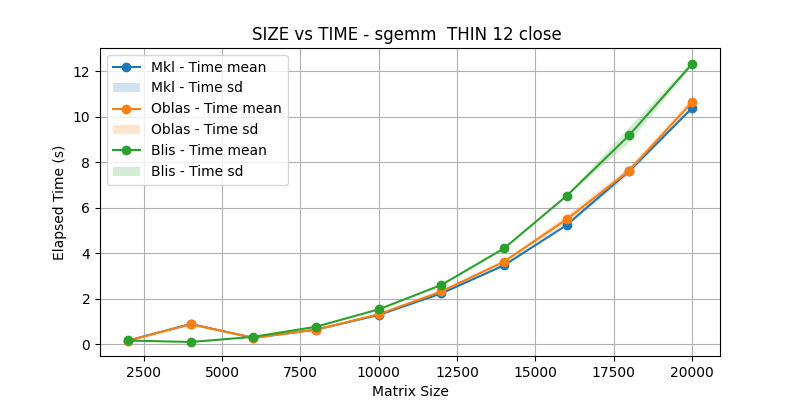
\includegraphics[width=\textwidth]{THIN 12/sgemm__THIN_12_close_time.png}
\end{figure}

As we can see, the MKL and OpenBLAS libraries are very similar in time terms while the BLIS library is a little bit slower for a size greater then 12000.

\begin{figure}[H]
    \centering
    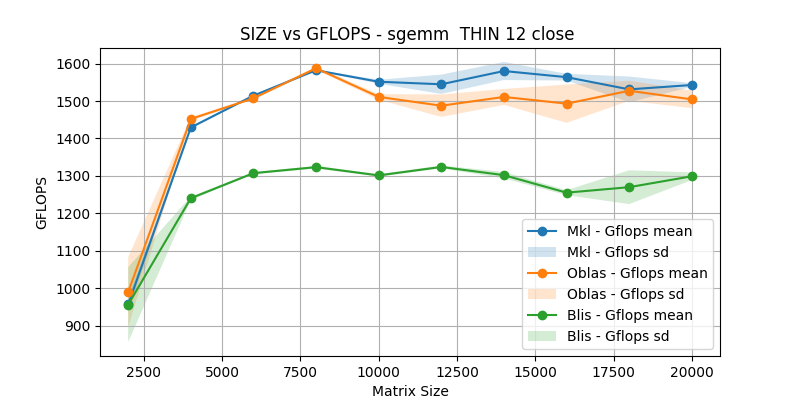
\includegraphics[width=\textwidth]{THIN 12/sgemm__THIN_12_close_gflops.png}
\end{figure}

As in the time study, the execution of the MKL and OpenBLAS libraries is similar, while the BLIS library allows to a smaller speed. In any case, we can see that with matrix sizes greater then 12000 we got a greater standard deviation in the experiments. 

 The plot below is still a test in single precision, but in this case we use the spread policy
\begin{figure}[H]
    \centering
    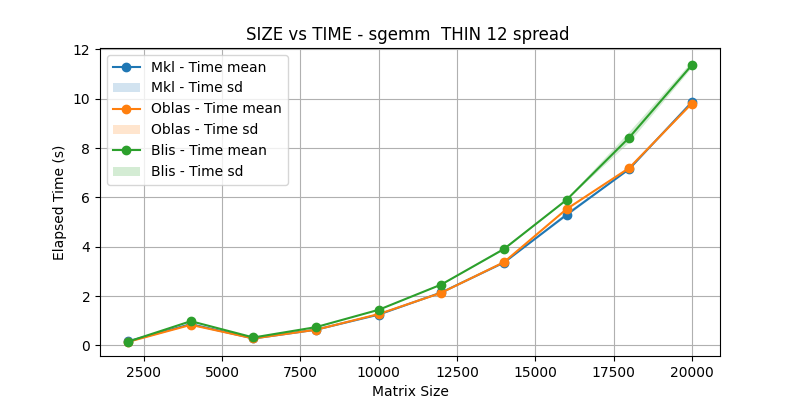
\includegraphics[width=\textwidth]{THIN 12/sgemm__THIN_12_spread_time.png}
\end{figure}

\begin{figure}[H]
    \centering
    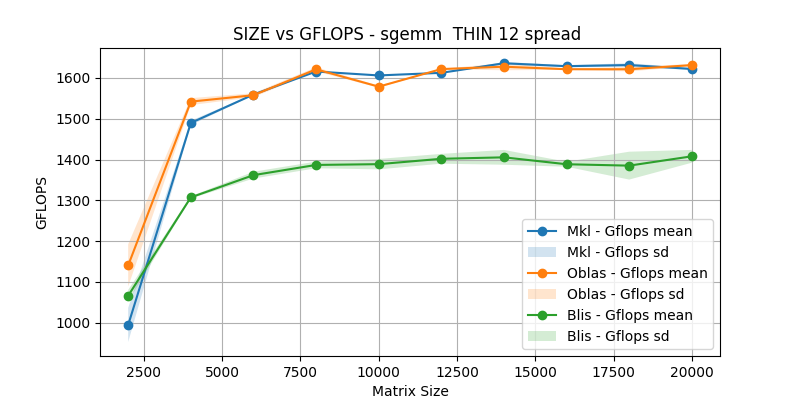
\includegraphics[width=\textwidth]{THIN 12/sgemm__THIN_12_spread_gflops.png}
\end{figure}

In times term, we have a similar results with respect to the close policy. However, it is interesting to see that the GFLOPS behavior of MKL and OpenBLAS in the spread case in much more similar w.r.t. the close policy.

Now, we repeated the previous tests, but in double precision.

\begin{figure}[H]
    \centering
    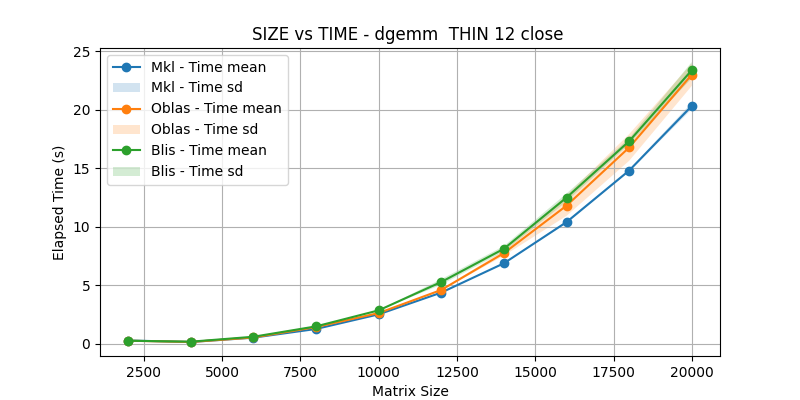
\includegraphics[width=\textwidth]{THIN 12/dgemm__THIN_12_close_time.png}
\end{figure}

\begin{figure}[H]
    \centering
    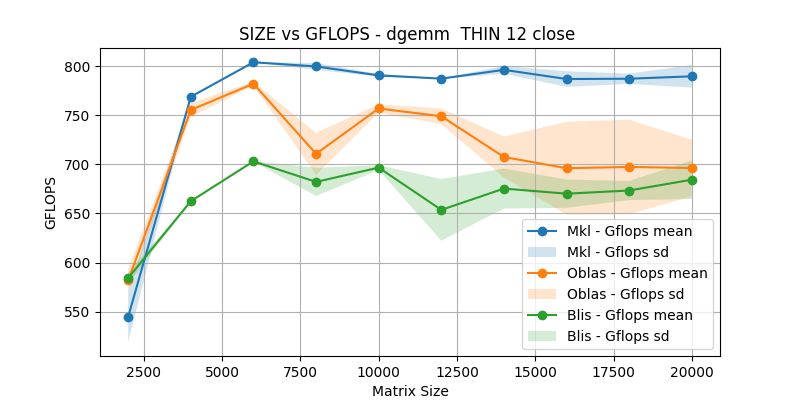
\includegraphics[width=\textwidth]{THIN 12/dgemm__THIN_12_close_gflops.png}
\end{figure}

In double precision the needed time is about twice the time of single precision, as we hoped, since it was coherent we our expectations. In this case, the greater speed was reached with the MKL library while with OpenBLAS the speed is similar to the blis one in case of big sizes. Furthermore, we can see the GFLOPS measures with OpenBLAS and BLIS have the biggest standard deviation seen w.r.t. all the previous cases studied.  

Finally, we tried the spread policy with double precision. In this case, we got a more clear behavior for the GFLOPS. As we can see in the following plots, the standard deviation is very small and we can state that the library with which we got the greater speed was MKL, followed by OpenBLAS, followed by BLIS.  

\begin{figure}[H]
    \centering
    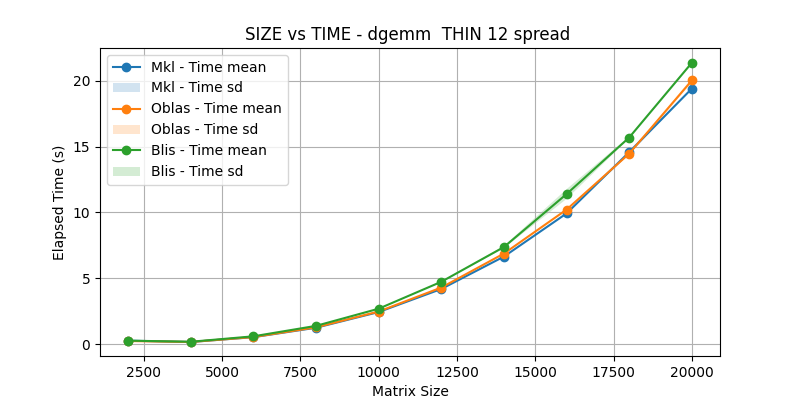
\includegraphics[width=\textwidth]{THIN 12/dgemm__THIN_12_spread_time.png}
\end{figure}

\begin{figure}[H]
    \centering
    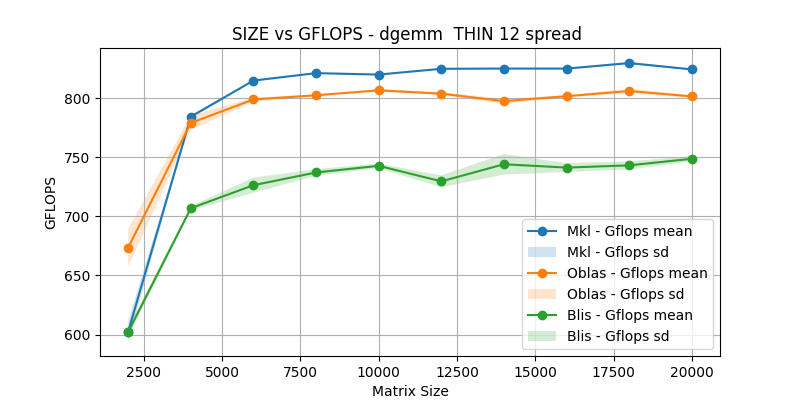
\includegraphics[width=\textwidth]{THIN 12/dgemm__THIN_12_spread_gflops.png}
\end{figure}



\subsubsection{Our peak performance}
The data:

With the THIN nodes, we reached the maximum performance in single precision with the MKL library on spread policy, when the size was 14000. The FLOPS were 1620.

For the double precision, we reached our maximum performance with MKL on spread policy, when the size was 18000. The FLOPS were 835. 

We concluded that, for the THIN nodes, with 12 cores, using spread policy and MKL library were the more important factors to reach the maximum performance. 

The optimized files: 

As we reported before, we try the command 
\begin{verbatim}
    -O3 -march=native
\end{verbatim}
in the compilation rules in order to increase the level of optimisation. Among all the trials, we chose to show the correspondent test on which in the previous files we reached the maximum performance so 
\begin{itemize}
    \item Single precision, spread policy
    \item Double precision, spread policy
\end{itemize}

For the single precision we can see that there is not a big difference.
\begin{figure}[H]
    \centering
    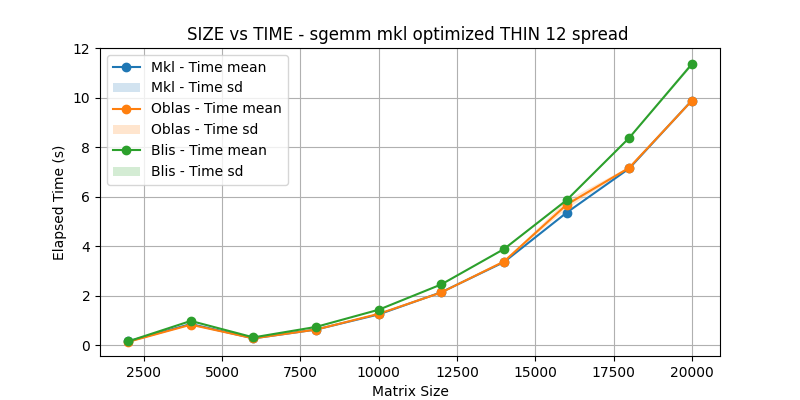
\includegraphics[width=\textwidth]{THIN 12/sgemm_mkl_optimized_THIN_12_spread_time.png}
\end{figure}

\begin{figure}[H]
    \centering
    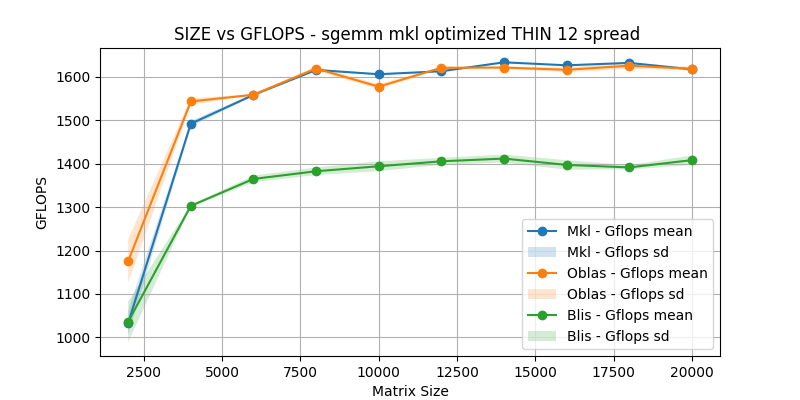
\includegraphics[width=\textwidth]{THIN 12/sgemm_mkl_optimized_THIN_12_spread_gflops.png}
\end{figure}

In the following plots, we plotted the results with the optimization steps. Here we can see that the GFLOPS are a little bit better then in the normal case but nothing special.  

\begin{figure}[H]
    \centering
    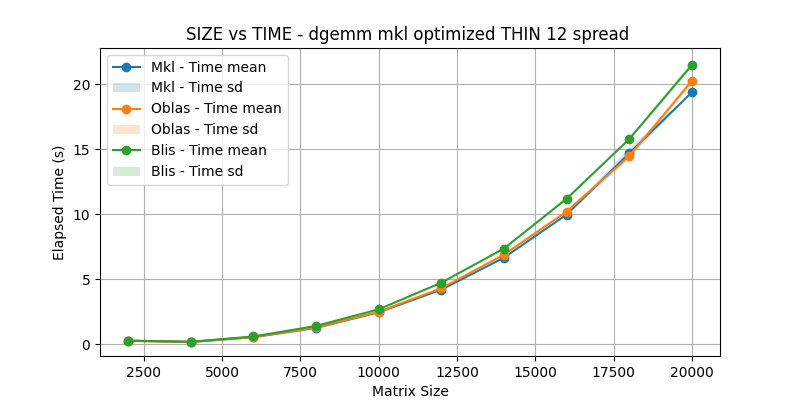
\includegraphics[width=\textwidth]{THIN 12/dgemm_mkl_optimized_THIN_12_spread_time.png}
\end{figure}

\begin{figure}[H]
    \centering
    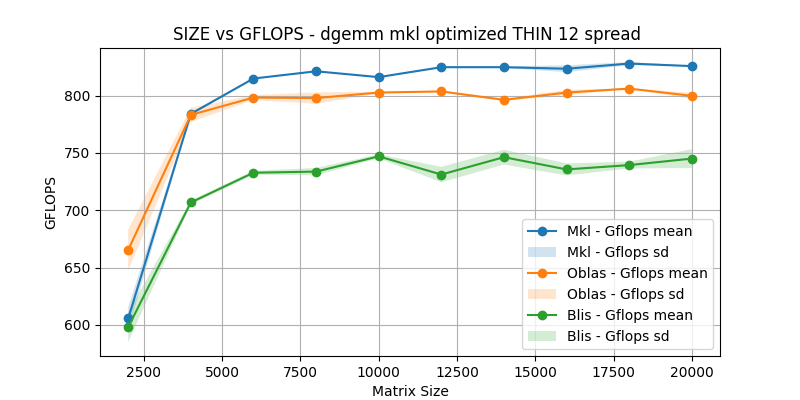
\includegraphics[width=\textwidth]{THIN 12/dgemm_mkl_optimized_THIN_12_spread_gflops.png}
\end{figure}

After the consideration of this section, we chose to omit the plots of the optimized libraries (they are in our GitHub anyway) since in the majority of the cases the were equal to the standard one and when they were better the improvement was very small.

\subsubsection{Results on fixed size}
In this sub subsection we will show our results regarding the strong scalability for the THIN nodes. As we discuss in the previous sections, our goal was to choose a size of the matrix in order to be enough big to appreciate the increase of speed when the used cores increases and sufficiently small to allow to an acceptable computation time. We had a threshold of 2 hours for each job, so we paid attention to avoid huge (relatively to our constraints) jobs. \
We chose a matrix size of 10000 and we increased the cpus from 1 to 24, by step of 2.
We started with close policy and single precision:
% Starting with "sgemm" and "close"
\begin{figure}[H]
    \centering
    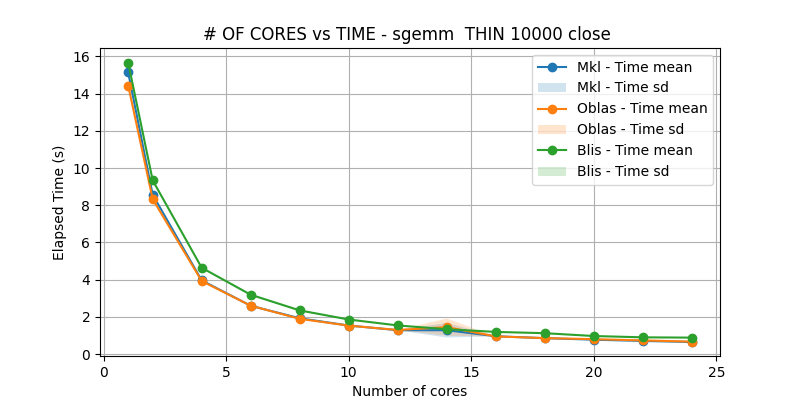
\includegraphics[width=\textwidth]{THIN scalability/sgemm__THIN_10000_close_time.png}
\end{figure}

\begin{figure}[H]
    \centering
    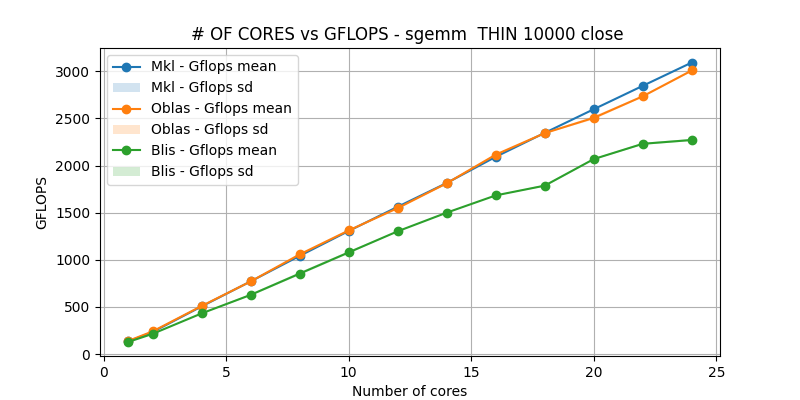
\includegraphics[width=\textwidth]{THIN scalability/sgemm__THIN_10000_close_gflops.png}
\end{figure}

We can see that the needed time drastically decreases when the cores go from 0 to 6. After 6 cores, the time continues to decrease, but more slowly. The GFLOPS have a clear linear growth on the number of cores.

% Replacing "close" with "spread"
Then, we did single precision tests with a spread policy.
\begin{figure}[H]
    \centering
    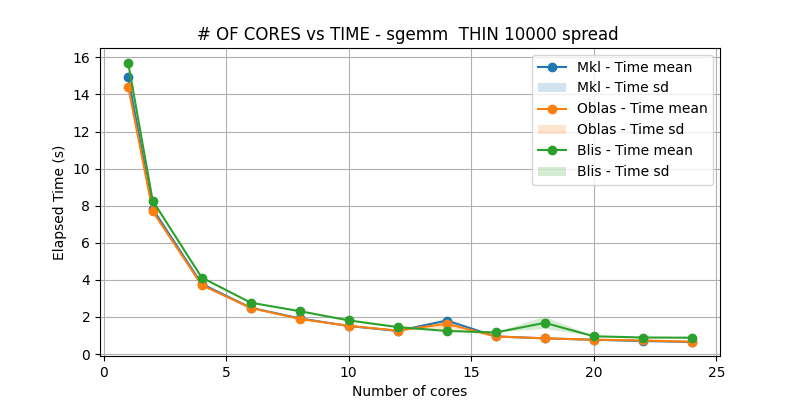
\includegraphics[width=\textwidth]{THIN scalability/sgemm__THIN_10000_spread_time.png}
\end{figure}

\begin{figure}[H]
    \centering
    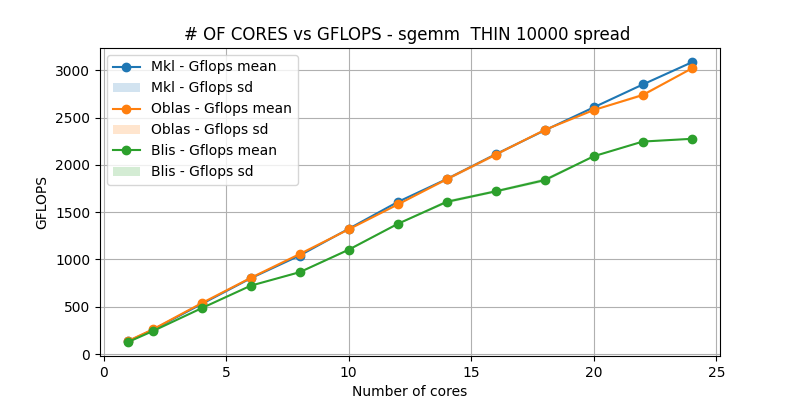
\includegraphics[width=\textwidth]{THIN scalability/sgemm__THIN_10000_spread_gflops.png}
\end{figure}

The results appears to be very similar to the close policy case. 

After, we tried the double precision.
% Replacing "sgemm" with "dgemm" and starting with "close"
\begin{figure}[H]
    \centering
    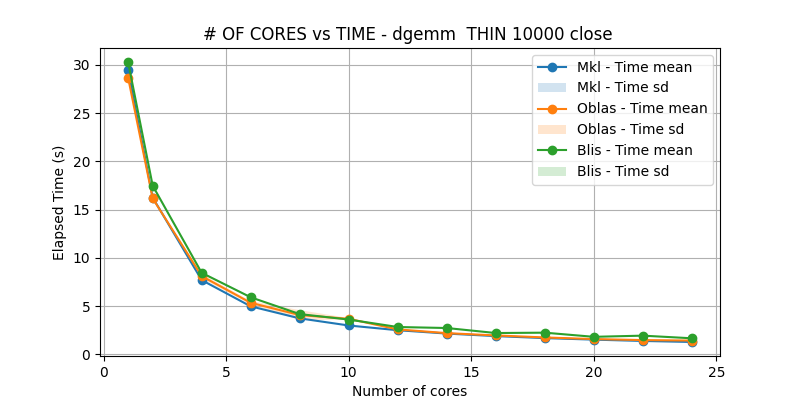
\includegraphics[width=\textwidth]{THIN scalability/dgemm__THIN_10000_close_time.png}
\end{figure}

\begin{figure}[H]
    \centering
    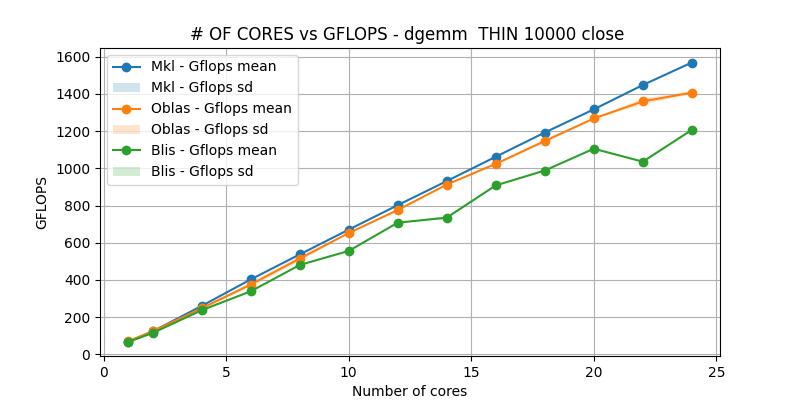
\includegraphics[width=\textwidth]{THIN scalability/dgemm__THIN_10000_close_gflops.png}
\end{figure}

Also in this case, we double the times w.r.t. single precision.

% spread
Finally, we tried the double precision with spread policy. As we can see in the following 2 plots all appears to be very similar to the previous case, but the behaviour of the GFLOPS in the BLIS case that is more regular.
\begin{figure}[H]
    \centering
    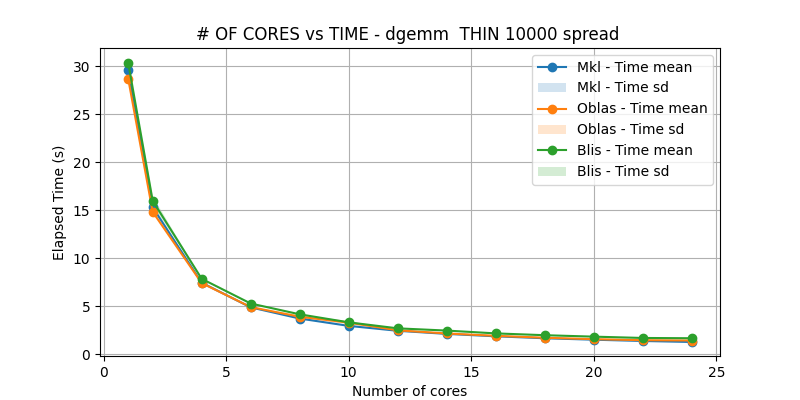
\includegraphics[width=\textwidth]{THIN scalability/dgemm__THIN_10000_spread_time.png}
\end{figure}

\begin{figure}[H]
    \centering
    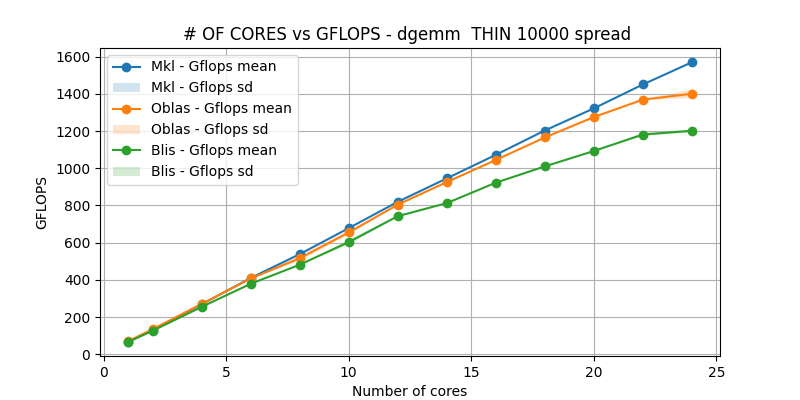
\includegraphics[width=\textwidth]{THIN scalability/dgemm__THIN_10000_spread_gflops.png}
\end{figure}

Now, since the big improvement of speed was from 1 to 6 cores, we focused on the range of cores from 1 to 10.

% Deep

% Starting with "sgemm" and "close"

We started with single precision and close policy. Differently from before, we can see in a clearer way the shape of the decrease of needed time when the used cores 
.   
\begin{figure}[H]
    \centering
    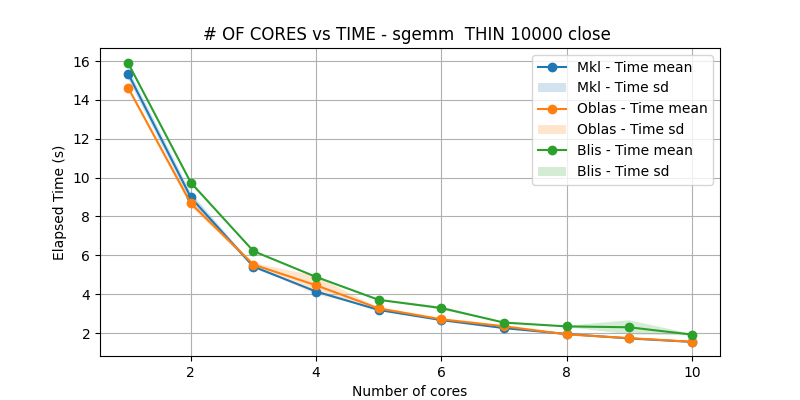
\includegraphics[width=\textwidth]{THIN scalability deep/sgemm__THIN_10000_close_time.png}
\end{figure}

\begin{figure}[H]
    \centering
    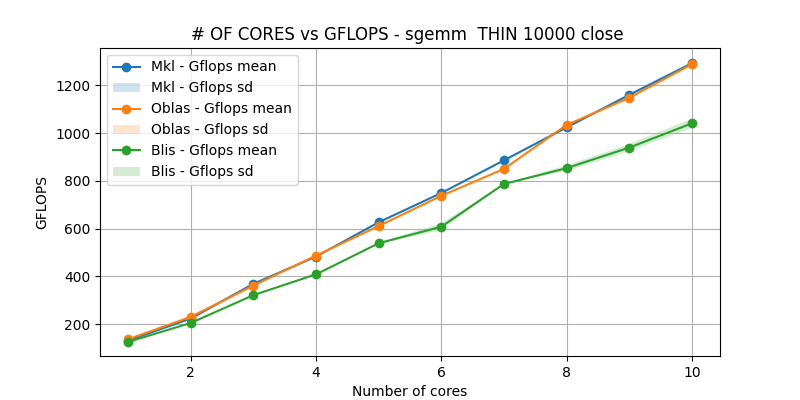
\includegraphics[width=\textwidth]{THIN scalability deep/sgemm__THIN_10000_close_gflops.png}
\end{figure}

% Replacing "close" with "spread"
Now we repeat the same thing, but with a spread policy.
\begin{figure}[H]
    \centering
    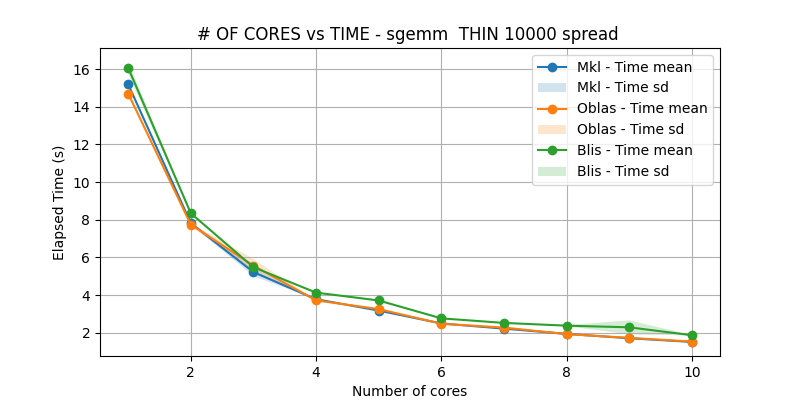
\includegraphics[width=\textwidth]{THIN scalability deep/sgemm__THIN_10000_spread_time.png}
\end{figure}

\begin{figure}[H]
    \centering
    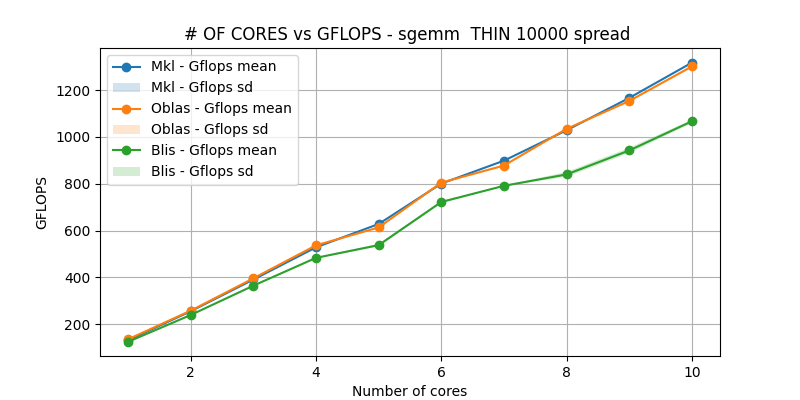
\includegraphics[width=\textwidth]{THIN scalability deep/sgemm__THIN_10000_spread_gflops.png}
\end{figure}

% Replacing "sgemm" with "dgemm" and starting with "close"
Finally, we completed the THIN case by studying the time and GFLOPS behaviours when the cores increase from 1 to 10, by a step of 1.
\begin{figure}[H]
    \centering
    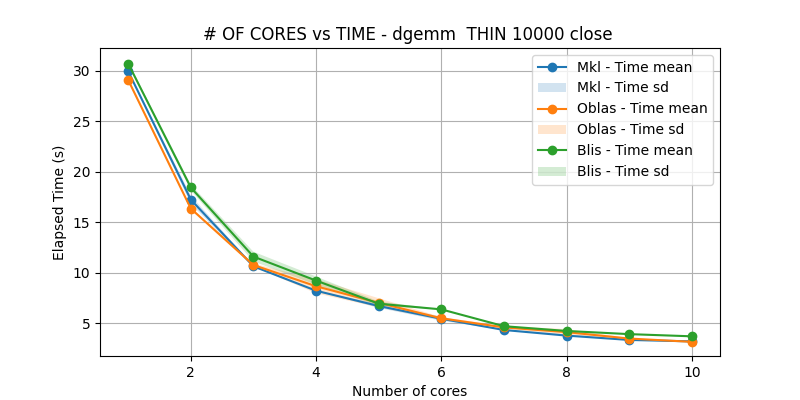
\includegraphics[width=\textwidth]{THIN scalability deep/dgemm__THIN_10000_close_time.png}
\end{figure}

\begin{figure}[H]
    \centering
    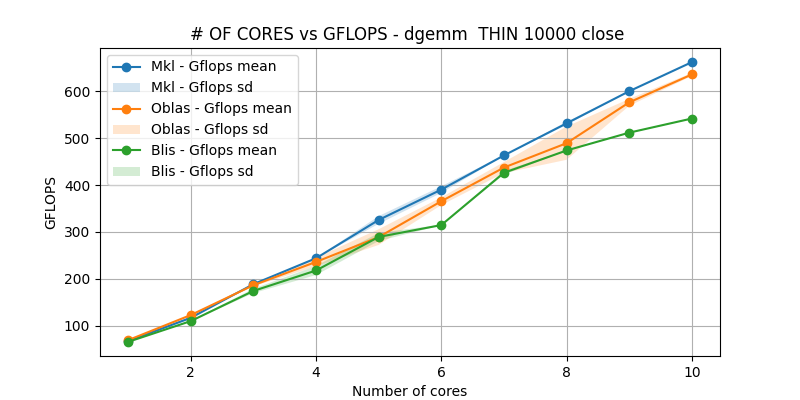
\includegraphics[width=\textwidth]{THIN scalability deep/dgemm__THIN_10000_close_gflops.png}
\end{figure}

% Replacing "close" with "spread"
\begin{figure}[H]
    \centering
    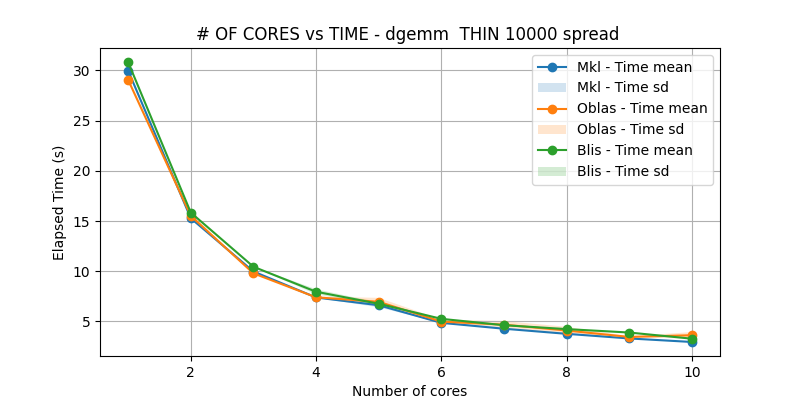
\includegraphics[width=\textwidth]{THIN scalability deep/dgemm__THIN_10000_spread_time.png}
\end{figure}

\begin{figure}[H]
    \centering
    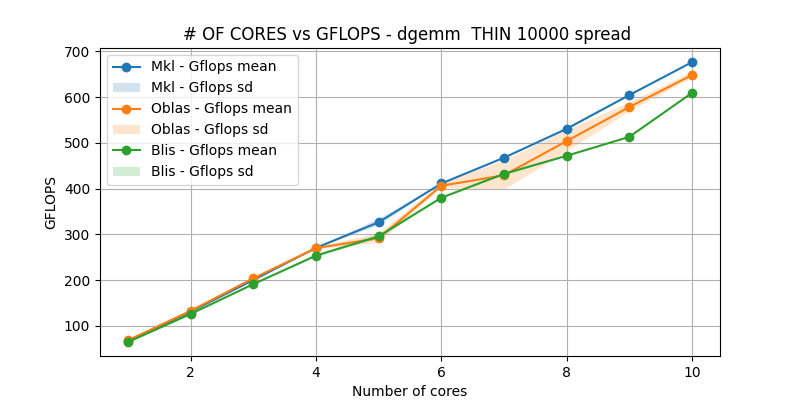
\includegraphics[width=\textwidth]{THIN scalability deep/dgemm__THIN_10000_spread_gflops.png}
\end{figure}

\subsubsection{The speed up}
As we discussed before, the speed up is a function on the size and on the number of processors that is equal to the serial time over the parallel time with $p$ processors on a size $n$.
The ideal speed up is serialTime/parallelTime = serialTime/serialTime/$p$ = $p$, where $p$ is the number of processors used. Then, we hope to be the more close as possible to the function $f(x) = x $ in the plot cores $\times$ speedUp.

We tried the single precision on close and spread policy: 
\begin{figure}[H]
    \centering
    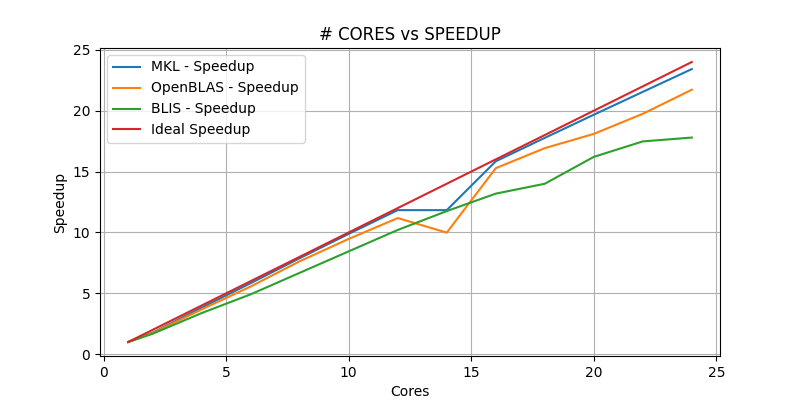
\includegraphics[width=\textwidth]{THIN speedUp/sgemm_mkl.x_THIN_10000_close_detailed__speedUp.png}
\end{figure}

\begin{figure}[H]
    \centering
    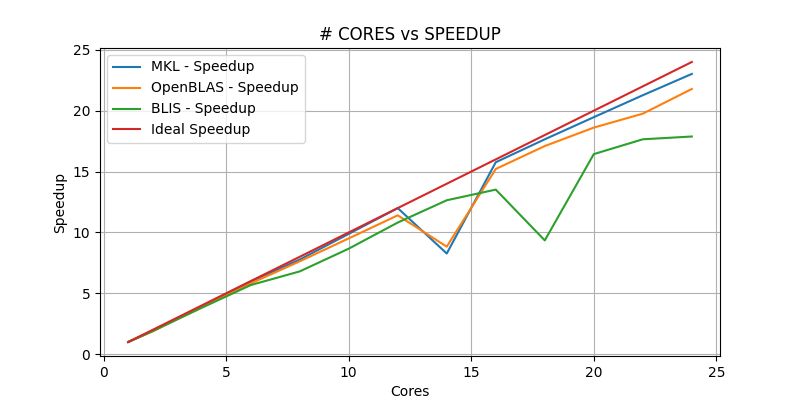
\includegraphics[width=\textwidth]{THIN speedUp/sgemm_mkl.x_THIN_10000_spread_detailed__speedUp.png}
\end{figure}

As we can see we are really close to the ideal speed up and it's a great thing. Especially the MKL library is the best.

Then, we tested the speed up for the double precision. The following plots shows that we have a situation simlar to the single precision. The MKL library continue to be the best in speed up term since it is very close to the ideal speed up.

Close policy:
\begin{figure}[H]
    \centering
    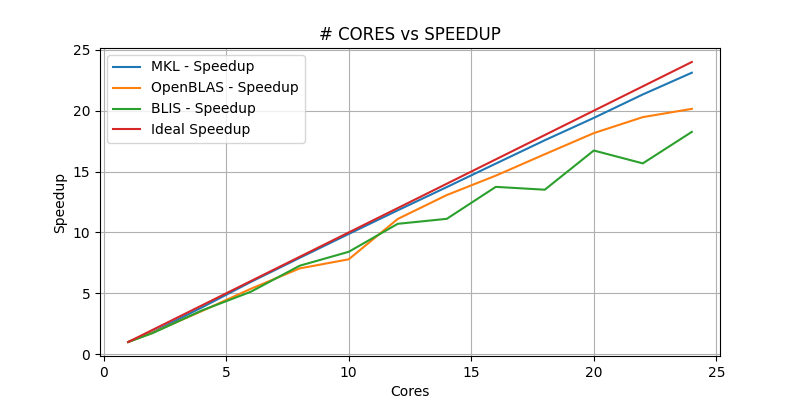
\includegraphics[width=\textwidth]{THIN speedUp/dgemm_mkl.x_THIN_10000_close_detailed__speedUp.png}
\end{figure}

Spread policy:
\begin{figure}[H]
    \centering
    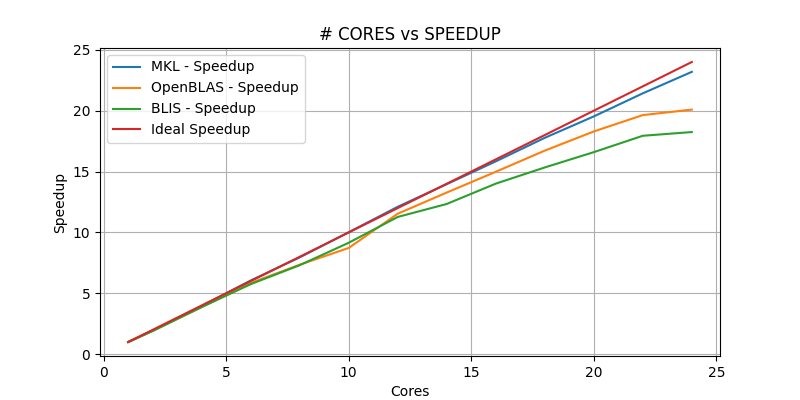
\includegraphics[width=\textwidth]{THIN speedUp/dgemm_mkl.x_THIN_10000_spread_detailed__speedUp.png}
\end{figure}

\subsection{EPYC case}
We tested the EPYC nodes and reported the results on this section. The schema was very similar to the previous section, but with a different focus on cores range in the strong scalability study. 

\subsubsection{Results on fixed number of cores}
An EPYC node has 128 cores in 2 sockets. Then we fixed a number of cores different from the THIN tests (now we used 64) and repeated the experiments for the MKL, OpenBLAS and BLIS libraries.   

First of all, we tested the three libraries with single precision and close policy.
\begin{figure}[H]
    \centering
    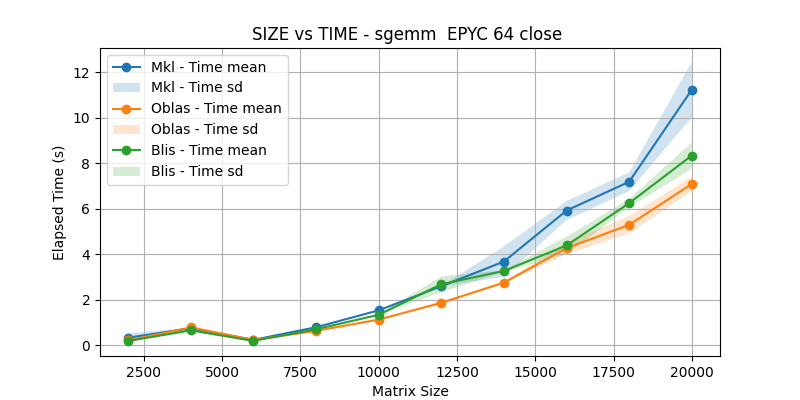
\includegraphics[width=\textwidth]{EPYC 64/sgemm__EPYC_64_close_time.png}
\end{figure}

\begin{figure}[H]
    \centering
    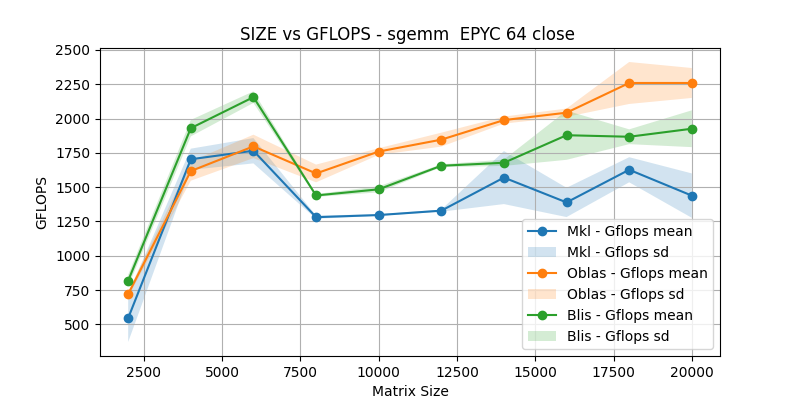
\includegraphics[width=\textwidth]{EPYC 64/sgemm__EPYC_64_close_gflops.png}
\end{figure}

It is very interesting to see that in this case the worst library, both in time and GFLOPS terms, is MKL. On the other hand, OpenBLAS is the best. In the THIN case the OpenBLAS was worse or close to the MKL. There is a big standard deviation, maybe because we did only 5 iterations for each size (instead of the 10 of the THIN nodes). 

In the following plots we tested the spread policy. 
\begin{figure}[H]
    \centering
    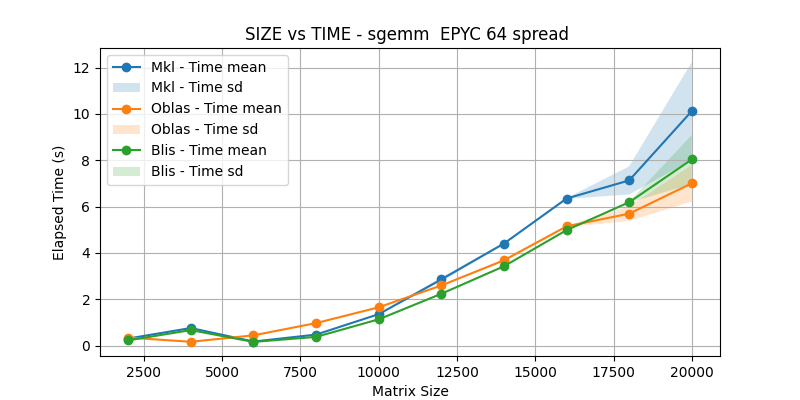
\includegraphics[width=\textwidth]{EPYC 64/sgemm__EPYC_64_spread_time.png}
\end{figure}

\begin{figure}[H]
    \centering
    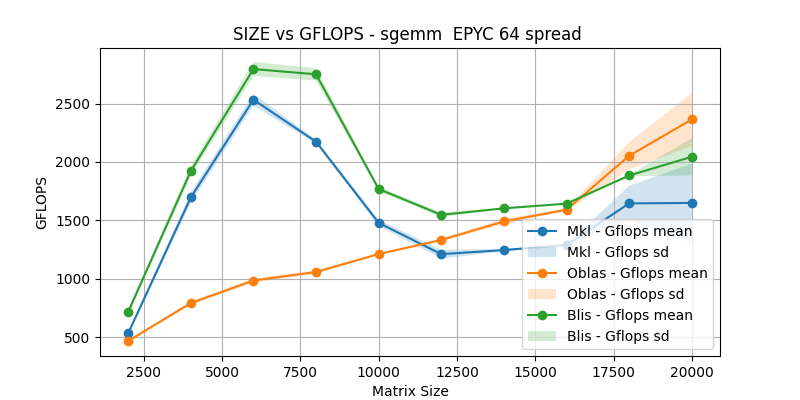
\includegraphics[width=\textwidth]{EPYC 64/sgemm__EPYC_64_spread_gflops.png}
\end{figure}

The spread case differs from the close case by a strange behaviours of the GFLOPS for the MKL and BLIS libraries and a clear and almost linear increase of GFLOPS for the OpenBLAS library. 

The, we tested the EPYC nodes with double precision. We started with a close policy.
\begin{figure}[H]
    \centering
    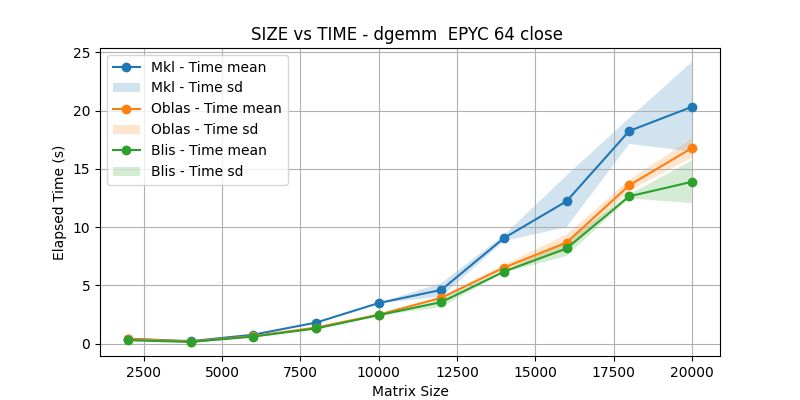
\includegraphics[width=\textwidth]{EPYC 64/dgemm__EPYC_64_close_time.png}
\end{figure}

\begin{figure}[H]
    \centering
    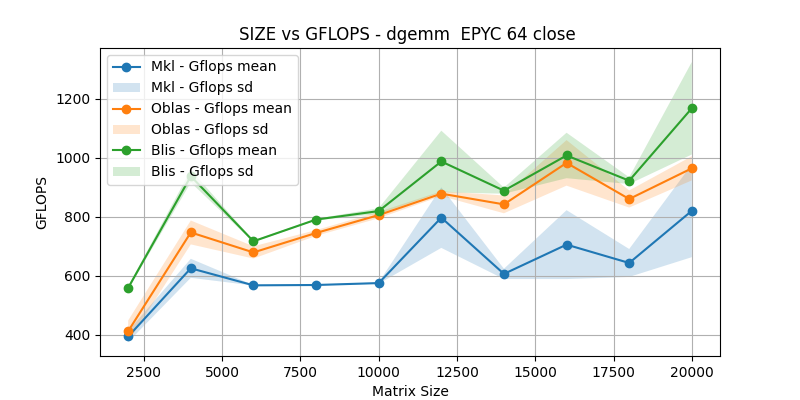
\includegraphics[width=\textwidth]{EPYC 64/dgemm__EPYC_64_close_gflops.png}
\end{figure}

It is notable that the blue line outperforms the red and blue lines (especially in GFLOPS terms). So, we found a case where the BLIS library appears to be the better. 

In order to conclude this sub section, we will show the case of double precision and spread policy. 
The graph illustrates similar times. The MKL appears to be a little bit better, but it has a greater standard deviation. 
\begin{figure}[H]
    \centering
    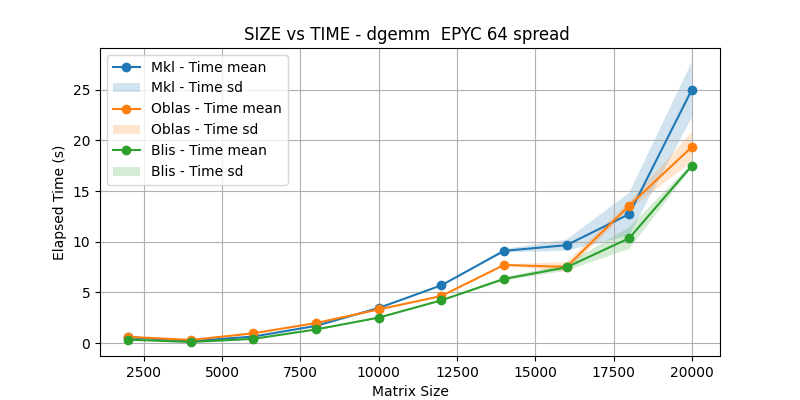
\includegraphics[width=\textwidth]{EPYC 64/dgemm__EPYC_64_spread_time.png}
\end{figure}

\begin{figure}[H]
    \centering
    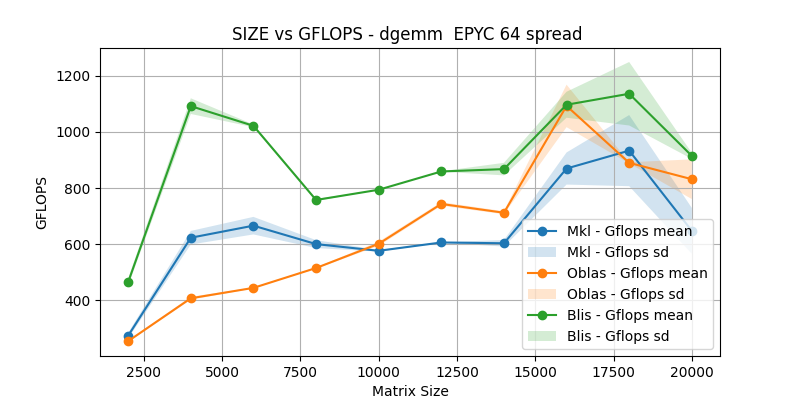
\includegraphics[width=\textwidth]{EPYC 64/dgemm__EPYC_64_spread_gflops.png}
\end{figure}

The data shows a steady domain of the BLIS library in GFLOPS terms. 

\subsubsection{Our peak performance}
For the EPYC nodes, we reached our peak performance for the single precision with the BLIS library and spread policy. Our peak performance was 2750 GFLOPS.

While, for the double precision, the peak performance was reached with BLIS library and close policy (1180 GFLOPS). We have to mention that with BLIS library and spread policy we were just a little bit below the 1180 GFLOPS, but we had a large standard deviation.

In any case, we can say that for the EPYC node the BLIS library is the best in order to reach the maximum performance. 

\subsubsection{Results on fixed size}
In this sub subsection we tested the strong scalability with the EPYC nodes. We fix a size of the matrix of 10000 in order to be consistent to the THIN studies. We increased the number of cores from 1 to 128 by steps of 16. We did more measures in the $[1,16]$ cores range, since is there then the time decreases the more.  

% Starting with "sgemm" and "close"
As usual, we started with single precision and close policy. 
\begin{figure}[H]
    \centering
    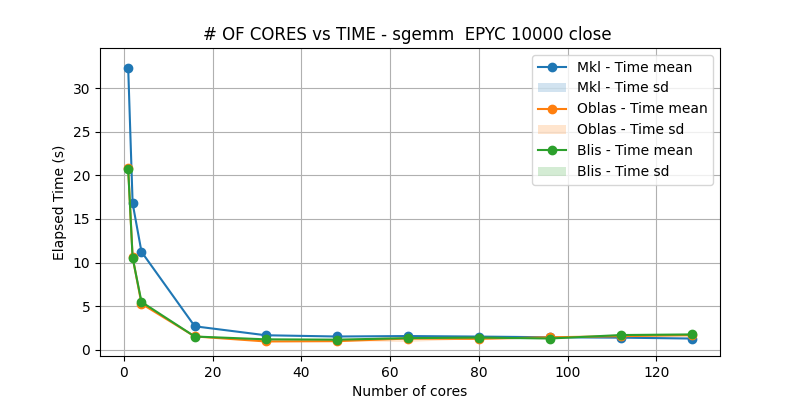
\includegraphics[width=\textwidth]{EPYC scalability/sgemm__EPYC_10000_close_time.png}
\end{figure}

\begin{figure}[H]
    \centering
    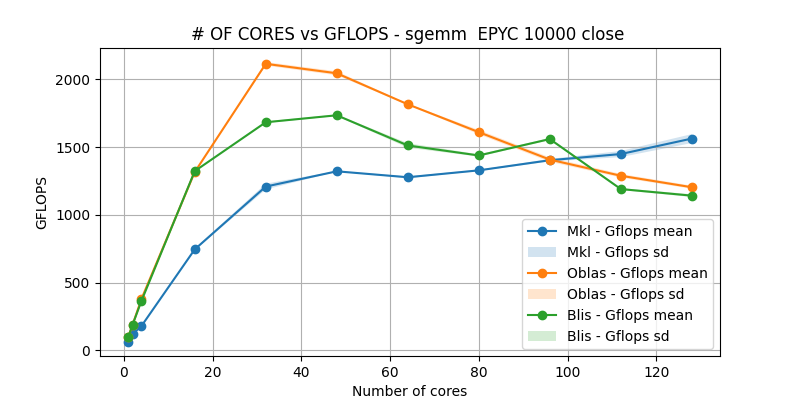
\includegraphics[width=\textwidth]{EPYC scalability/sgemm__EPYC_10000_close_gflops.png}
\end{figure}
In the chart, we can see an immediate and sudden decrease of execution time. While we observe a peak of GFLOPS when the number of cores is around 40. 

% Replacing "close" with "spread"
We did the same tests, but with spread policy.
\begin{figure}[H]
    \centering
    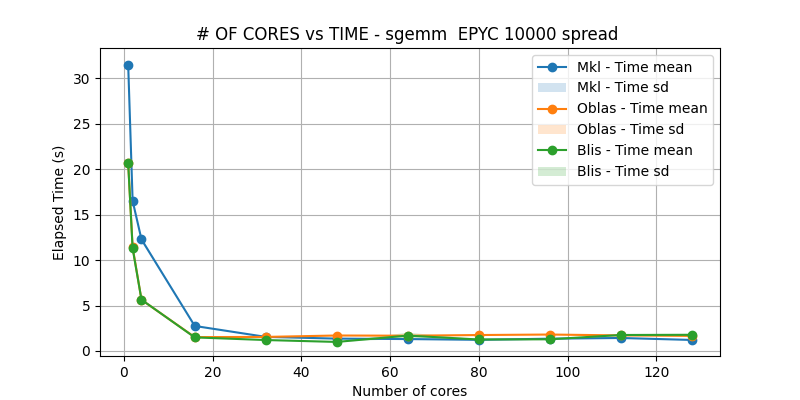
\includegraphics[width=\textwidth]{EPYC scalability/sgemm__EPYC_10000_spread_time.png}
\end{figure}

\begin{figure}[H]
    \centering
    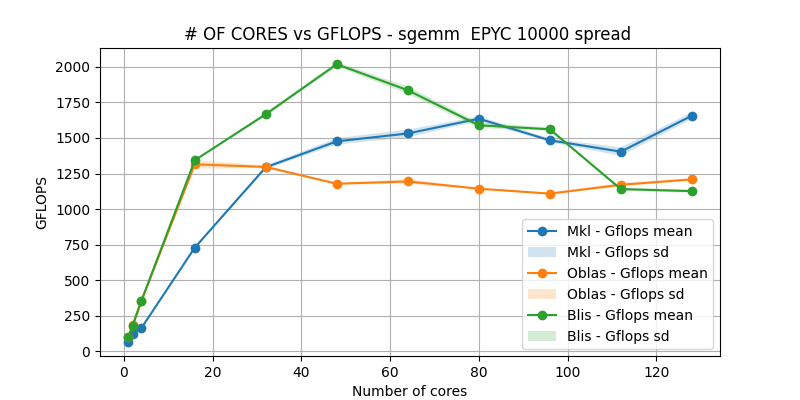
\includegraphics[width=\textwidth]{EPYC scalability/sgemm__EPYC_10000_spread_gflops.png}
\end{figure}
In contrast to the close policy,the spread policy exhibits a lower pick of performance of the OpenBLAS library. 

% Replacing "sgemm" with "dgemm" and starting with "close"
After, we tried the double precision.
\begin{figure}[H]
    \centering
    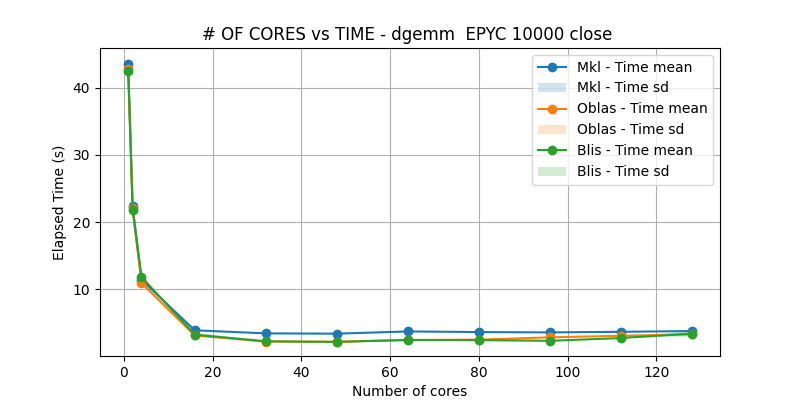
\includegraphics[width=\textwidth]{EPYC scalability/dgemm__EPYC_10000_close_time.png}
\end{figure}

\begin{figure}[H]
    \centering
    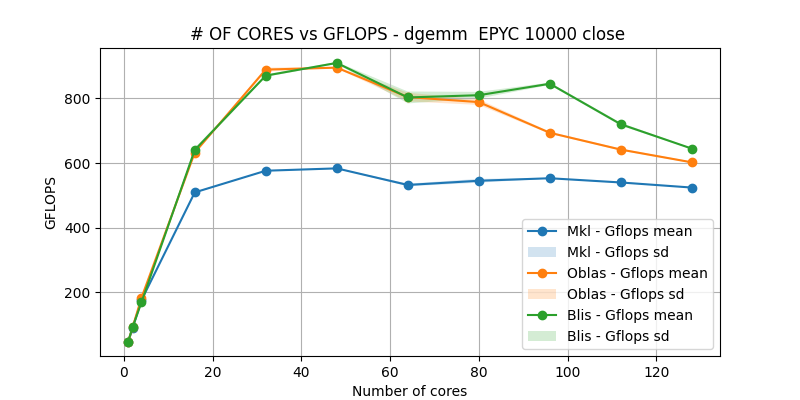
\includegraphics[width=\textwidth]{EPYC scalability/dgemm__EPYC_10000_close_gflops.png}
\end{figure}

It is interesting to note that the MKL library is worse then the others in both times and GFLOPS terms.

% Replacing "close" with "spread"
This plot presents data on the spread policy.
\begin{figure}[H]
    \centering
    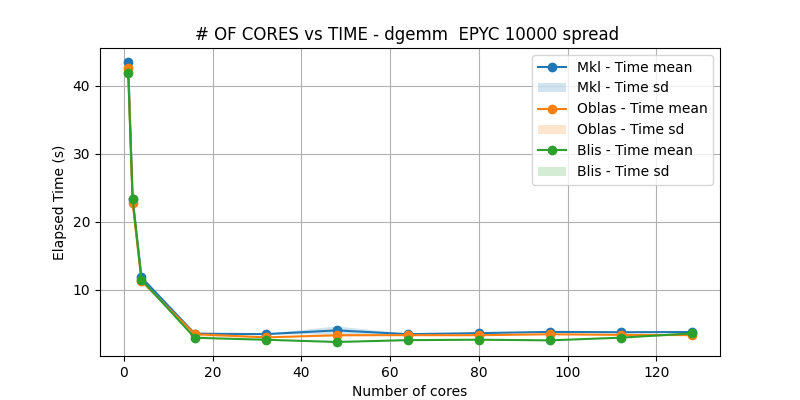
\includegraphics[width=\textwidth]{EPYC scalability/dgemm__EPYC_10000_spread_time.png}
\end{figure}

\begin{figure}[H]
    \centering
    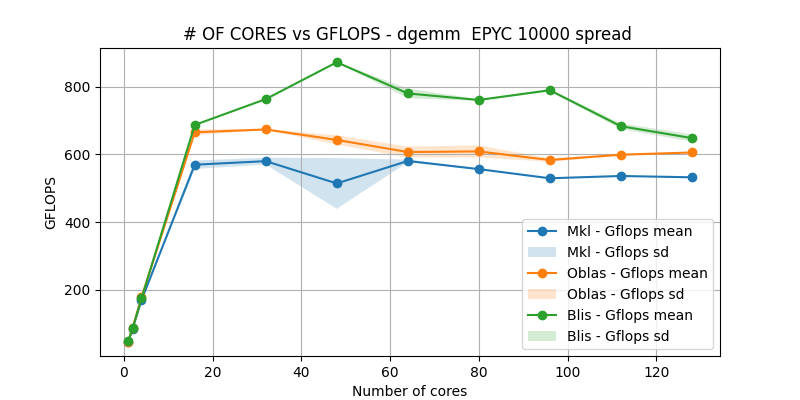
\includegraphics[width=\textwidth]{EPYC scalability/dgemm__EPYC_10000_spread_gflops.png}
\end{figure}
In this case, there is a clear upward trend of the BLIS library.

In order to conclude the EPYC study, we wanted to focused on the $[1,16]$ range for the cores.
This plot presents data on single precision with close policy.
% Starting with "sgemm" and "close"
\begin{figure}[H]
    \centering
    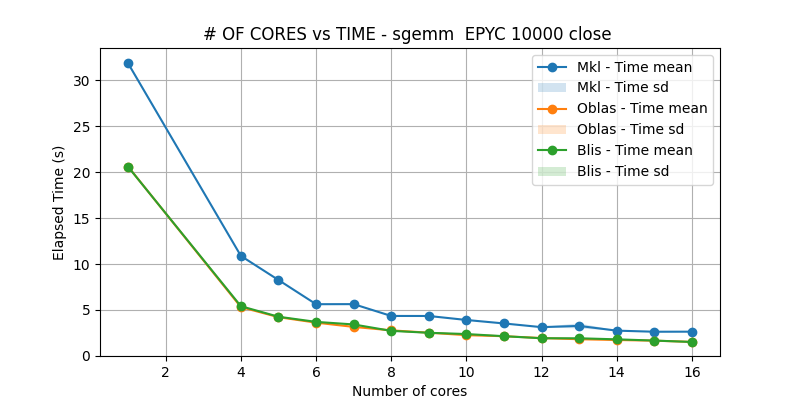
\includegraphics[width=\textwidth]{EPYC scalability deep/sgemm__EPYC_10000_close_time.png}
\end{figure}

\begin{figure}[H]
    \centering
    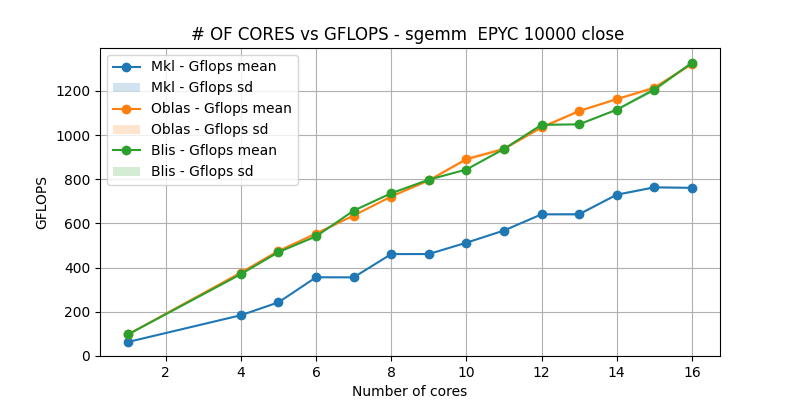
\includegraphics[width=\textwidth]{EPYC scalability deep/sgemm__EPYC_10000_close_gflops.png}
\end{figure}
Now there is a clearer view of the worse performance of the MKL library. 

% Replacing "close" with "spread"
We got similar result for the spread policy.
\begin{figure}[H]
    \centering
    \includegraphics[width=\textwidth]{EPYC scalability deep/sgemm__EPYC_10000_spread_time.png}
\end{figure}

\begin{figure}[H]
    \centering
    \includegraphics[width=\textwidth]{EPYC scalability deep/sgemm__EPYC_10000_spread_gflops.png}
\end{figure}

% Replacing "sgemm" with "dgemm" and starting with "close"
The figure provides an overview of the tests on double precision.
\begin{figure}[H]
    \centering
    \includegraphics[width=\textwidth]{EPYC scalability deep/dgemm__EPYC_10000_close_time.png}
\end{figure}

\begin{figure}[H]
    \centering
    \includegraphics[width=\textwidth]{EPYC scalability deep/dgemm__EPYC_10000_close_gflops.png}
\end{figure}

In this case, there appears to be a similarity between the three libraries.

% Replacing "close" with "spread"
A really analogous behaviour in the spread policy cases.
\begin{figure}[H]
    \centering
    \includegraphics[width=\textwidth]{EPYC scalability deep/dgemm__EPYC_10000_spread_time.png}
\end{figure}

\begin{figure}[H]
    \centering
    \includegraphics[width=\textwidth]{EPYC scalability deep/dgemm__EPYC_10000_spread_gflops.png}
\end{figure}



\clearpage % Start a new page for the index.

% Index section
\printindex

\end{document}
